% -----------------------------------------------
% Template for ISMIR Papers
% 2015 version, based on previous ISMIR templates
% -----------------------------------------------

\documentclass{article}
\usepackage{ismir,amsmath,cite}
\usepackage{graphicx}
\usepackage{color}

% Title.
% ------
\title{Chroma Convolution Method: an alternative for chroma feature construction}

% Single address
% To use with only one author or several with the same address
% ---------------
%\oneauthor
% {Names should be omitted for double-blind reviewing}
% {Affiliations should be omitted for double-blind reviewing}

% Two addresses
% --------------
%\twoauthors
%  {First author} {School \\ Department}
%  {Second author} {Company \\ Address}

% Three addresses
% --------------
\threeauthors
 {} {\\ {\tt }}
  {} {\\ {\tt}}
  {} {\\ {\tt}}

  %{Jose Pedro de Santana Neto} {University of Brasilia - FGA\\ {\tt 1jpsneto@gmail.com}}
  %{Henrique Gomes de Moura} {University of Brasilia - FGA\\ {\tt hgmoura@yahoo.com}}
  %{Fernando William Cruz} {University of Brasilia - FGA\\ {\tt fwcruz@unb.br}}

% Four addresses
% --------------
%\fourauthors
%  {First author} {Affiliation1 \\ {\tt author1@ismir.edu}}
%  {Second author}{Affiliation2 \\ {\tt author2@ismir.edu}}
%  {Third author} {Affiliation3 \\ {\tt author3@ismir.edu}}
%  {Fourth author} {Affiliation4 \\ {\tt author4@ismir.edu}}

\begin{document}
%
\maketitle
%
\begin{abstract}

This paper is presented as an alternative and efficient method to the construction of the chroma feature or Pitch Class Profile (PCP). Chroma Convolution Method (CCM), which is an operation essentially in the time domain, embodies peculiar characteristics that optimize the distinctions of musical tones and timber in musical instruments. For the demonstration of the efficacy of this method, comparative experiments with the traditional method, DFT or STFT,  were made. The experiments have shown that CCM is the most efficient in the identification of musical tones; moreover, it holds the capacity of distinguishing musical tones of different musical instruments, when they are also played at the same time.
\end{abstract}
%
\section{Introduction}\label{sec:introduction}

% 1- problema

	The process of extraction of chroma feature is a steady matter in solutions of automatic music transcription. Basically, this process consists in obtaining the spectrum of frequency in audio signals, and also calculating the level of energy of each one of the 12 tones that are part of the temperament scale. Traditionally, the Fourier transform is used for this extraction since about 1999 with Fujishima \cite{fujishima1999realtime}, and, since then, a great effort is being made in order to optimize the Pitch Class Profile (PCP), built by the discrete Fourier transform (DFT).

	Many studies approach the matter of construction of chrome feature in music. These studies have built solutions which are based on DFT and STFT (Short Time Fourier Transform) to the identification of melodies: \cite{muto2002transcription}, \cite{al2008time}, \cite{barbancho2009transcription}, \cite{gomez2004automatic}, \cite{tangmelody}, \cite{eggink2004extracting} and \cite{jo2010melody}, this last one appling optimizations, by using particle filters. Also, there are some chroma feature studies which focus on the automatic transcription of chords via DFT:
	\cite{harte2009automatic}, \cite{khadkevich2011time}, \cite{harte2010towards}, \cite{peeters2006chroma}, \cite{cho2010exploring} \cite{lee2006automatic}, \cite{de2012improving}, \cite{boulanger2013audio}, \cite{chen2012chord} and \cite{hrybyk2010combined}.

% 3- deficiencias nos estudos
The aforementioned studies focus on adapted version of the DFT, has there are not many alternatives of tones characterization, besides the DFT. There are again many DFT limitations, quoted in papers like Harte's \cite{harte2010towards}. The study of Mauch \cite{mauch2010approximate} for instance, focus on the application of NNLS to the increasement of identification of tones, and paper \cite{wakefield1999mathematical} focus on the mathematical model to the representation of tones distributions and its frequencies. However, there still is the need of alternative methods in relation to DFT and the construction of chroma feature.

% 4- importancia do estudo para o publico
It is shown on this paper an alternative method for chroma feature caracterization and melodies identification, in time domain. The Chroma Convolution Method (CCM) embodies peculiar characteristics that optimize the distinctions of musical tones and timber in musical instruments. The CCM can replace the DFT or STFT to extract polyphonic sounds with more accuracy, as well as identifying tones of different musical instruments.

	This paper has been organized in the following way: Section 2 describes the use, general aspects and limitations of DFT; Section 3 presents the conceptualization of the suggested method, characteristics and the process of construction of chroma feature using CCM; Section 4 presents two comparative experiments, of DFT and CCM methods; Section 5 delimits discussions about the results of CCM's efficacy; Section 6 presents conclusions and further papers. 

\section{Discrete Fourier Transform (DFT)}\label{sec:sfft}

	Chroma feature or pitch class profile (PCP) have been exclusively used as an front-end to the recognition of chords or extraction of melodies of recorded audio. Fujishima \cite{fujishima1999realtime} developed a system of automatic transcription of chords in real-time, where he derives a chroma feature in 12 dimensions from the DFT audio signal. Since then, the Discrete Fourier Transform (DFT or FFT) has been used to the construction of chromatic features the audio. The function of this transform is translating pieces of information which are in time domain to frequency domain in a way to project, in orthonormal basis, the value of each sine component present in the signal in question. This projection results of the sum of inner sines (complex exponentials) products, by the signal \cite{vaidyanathan1993multirate}.

	Since this transform only offers information in terms of frequency, the need of adapting it to the visualization of the variation of frequency through time has taken place. This adaption is called short time fourier transform (STFT) \cite{cohen1995time}. In a nutshell, this process of windowing consists of dividing the signal in parts to be analyzed individually in the frequency domain, which means that in each minute-time that refers to each sound clip it is possible to obtain frequency analysis.

	However, this technique presents some limitations:
	\begin{itemize}
		\item the appearance of aliasing that can make the identification of actually played tones difficult;
		\item problems of spectral leakage, generated from signal truncation, possibly causing frequencies that make the spectrum visualization more difficult;
		\item problems in the determination of the window length, as the sampling parameter can limit the frequency band to be analyzed.
	\end{itemize}

	It can be observed that the presented limitations are, mostly, originated from the digital processing of signals necessary to the constitution of frequency spectrum. Being so, one might research on alternatives for this problem of chroma feature construction in the frequency domain, in order to preserve the original characteristics of audio signals.

\section{Chroma Convolution Method (CCM)}\label{sec:ccm}

	The chroma convolution method (CCM) aims to project the sound passage of the sign on each one of the tones sought. It can be observed that when the sign to be processed is projected on the sign of a musical note, through convolution, the sound of the first tone is amplified and the others are suppressed. 

	Let's take a note formed from a monochromatic sine. When this sign is convoluted with processed audio sign it is possible to extract as a result the level of energy related to that frequency.  This energy is measured through the following \eqnref{ccm_equation} equation:

	\begin{equation}\label{ccm_equation}
		E = \sum [f(x)*g(x)]^{2}
	\end{equation}

	In this context, the chroma features were built from the following procedures:
	\begin{enumerate}
		\item the audio was divided to be analyzed in signals with pre-determined duration;
		\item monochromatic sine functions were used to build musical tones in time domain, corresponding to the chromatic musical scale;
		\item each part of the audio signal was convoluted with the musical tones;
		\item the convolution energy was extracted from the equation \eqnref{ccm_equation};
		\item Finally, each energy was summed up with the respective eights, originating the chroma feature, presented in a schema on \figref{fig:chroma_feature}.
	\end{enumerate}

	
	\begin{figure}[h!]
		 \centerline{\framebox{
		 \includegraphics[width=\columnwidth, height=6cm]{figs/chroma_feature.png}}}
		 \caption{Schematic representation of the chroma feature. On this chart, a full chromatic scale starting from A up to G\#.}
		 \label{fig:chroma_feature}
		\end{figure}

	\figref{fig:schematic} represents a schematic point of view of the proceeding described. By the end of the process, the chroma features can be visualized from an spectrogram of 12 dimensions.

	\begin{figure}[h!]
	 \centerline{\framebox{
	 \includegraphics[width=\columnwidth]{figs/schematic.png}}}
	 \caption{Schematic of process to build chroma feature using CCM.}
	 \label{fig:schematic}
	\end{figure}


\section{Experiments and Results}

	In order to proove the efficacy of CCM in relation to the traditional method STFT \cite{LabROSA}, in what concerns the identification of tones played from their chroma features, 2 experiments were made, using MATLAB as programming language. Recorded audio signals of actual musical instruments were used as data entry. MIREX\footnote{http://www.music-ir.org/mirex/wiki/MIREX\_HOME} was not used because such experiments needed a bigger control over audio execution, considering a common acoustic environment, but both techniques were compared under the same audio database\footnote{Code and audio recorded available in https://github.com/josepedro/ismir\_article.}. 

	
	\subsection{Experiment 1: Identification of Musical Notes}

	The first experiment is about the identification of musical tones in a piano melody. Those tones were played according to \figref{fig:1-notes}.

	\begin{figure}[h!]
	 \centerline{\framebox{
	 \includegraphics[width=\columnwidth]{figs/1-notes.png}}}
	 \caption{Recorded notes played on piano.}
	 \label{fig:1-notes}
	\end{figure}

	Convolution with 96 pure tones of different frequency was used to generate the chroma feature in CCM results. The windows of both proposals were set in the length of 0.120 seconds and the samplings rate of the audio was of 44.1 kHz.

	\subsubsection{STFT Results}
	In the following, chroma feature found using the traditional method of STFT in \figref{fig:1-ssft}. It can be observed that the chromatic scale was identified, yet with some discrepancies in relation to the exact moment that the tones were played. One can notice, for example, that one tone E was identified in the beginning as, in reality, it should be identified in about 7 seconds. 

	
	\begin{figure}[h!]
	 \centerline{\framebox{
	 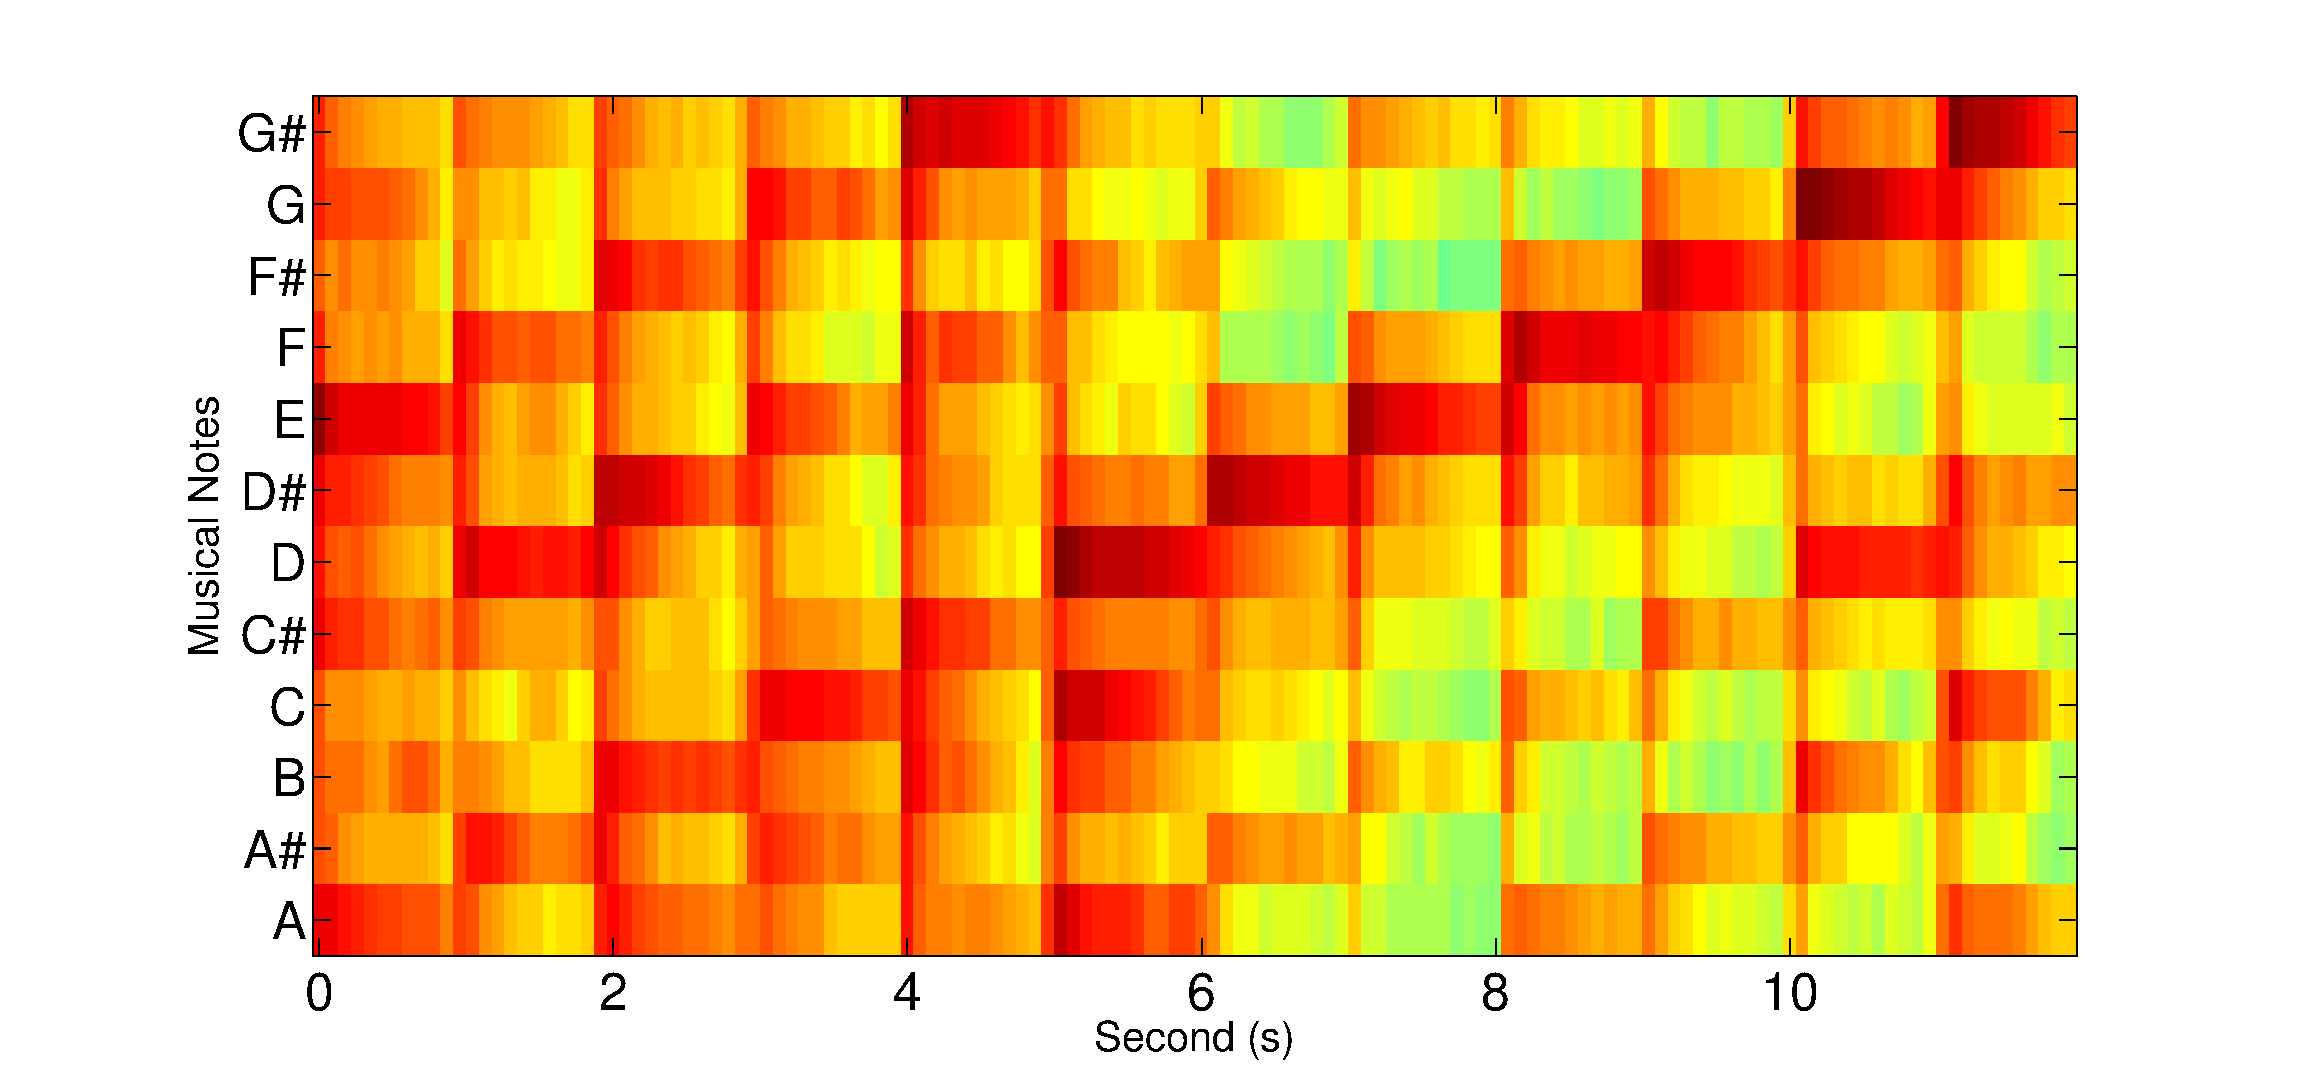
\includegraphics[width=\columnwidth, height=6cm]{figs/1-sfft.eps}}}
	 \caption{Obtained chroma feature by using the STFT method.}
	 \label{fig:1-ssft}
	\end{figure}	

	
	An efficiency analysis of the tones recorded in audio with the sequence of tones identified in the chroma feature was also made. The identified tones were selected thorough the highest intensity in each minute-time. \tabref{tab:table-1-sfft} represents the tones which were played and also the ones which were identified in the chroma feature. There were 9 out of 14 tones playing in the correct moment, so, 64.3\% of fidelity to the original melody.  

	

	\begin{table}[h!]
	 \begin{center}
	 \begin{tabular}{|l|l|}
	  \hline
	  Played Notes & Identified Notes \\
	  \hline
	  A  & E \\
	  A\#  & D \\
	  A\#  & D\# \\
	  B  & B \\
	  B\#  & E \\
	  C  & D \\
	  C\#  & G\# \\
	  D  & D \\
	  D\#  & D\# \\
	  E  & E \\
	  F  & F \\
	  F\#  & F\# \\
	  G  & G \\
	  G\#  & G\# \\
	  \hline
	 \end{tabular}
	\end{center}
	 \caption{Comparison between played and identified notes by the STFT method.}
	 \label{tab:table-1-sfft}
	\end{table}

	


	\subsubsection{CCM Results}
	Chroma feature found using CCM on \figref{fig:1-ccm}. It can be observed that the melody represented itself more clearly. A comparative table of the played and identified tones was made through the extraction of the tone of the chroma feature with more intensity in each minute-time. Keeping in mind the results of \tabref{tab:table-1-ccm}, 13 out of 14 tones were playing in the correct moment, so, 92.9\% fidelity to the original melody.
	
	\begin{figure}[h!]
	 \centerline{\framebox{
	 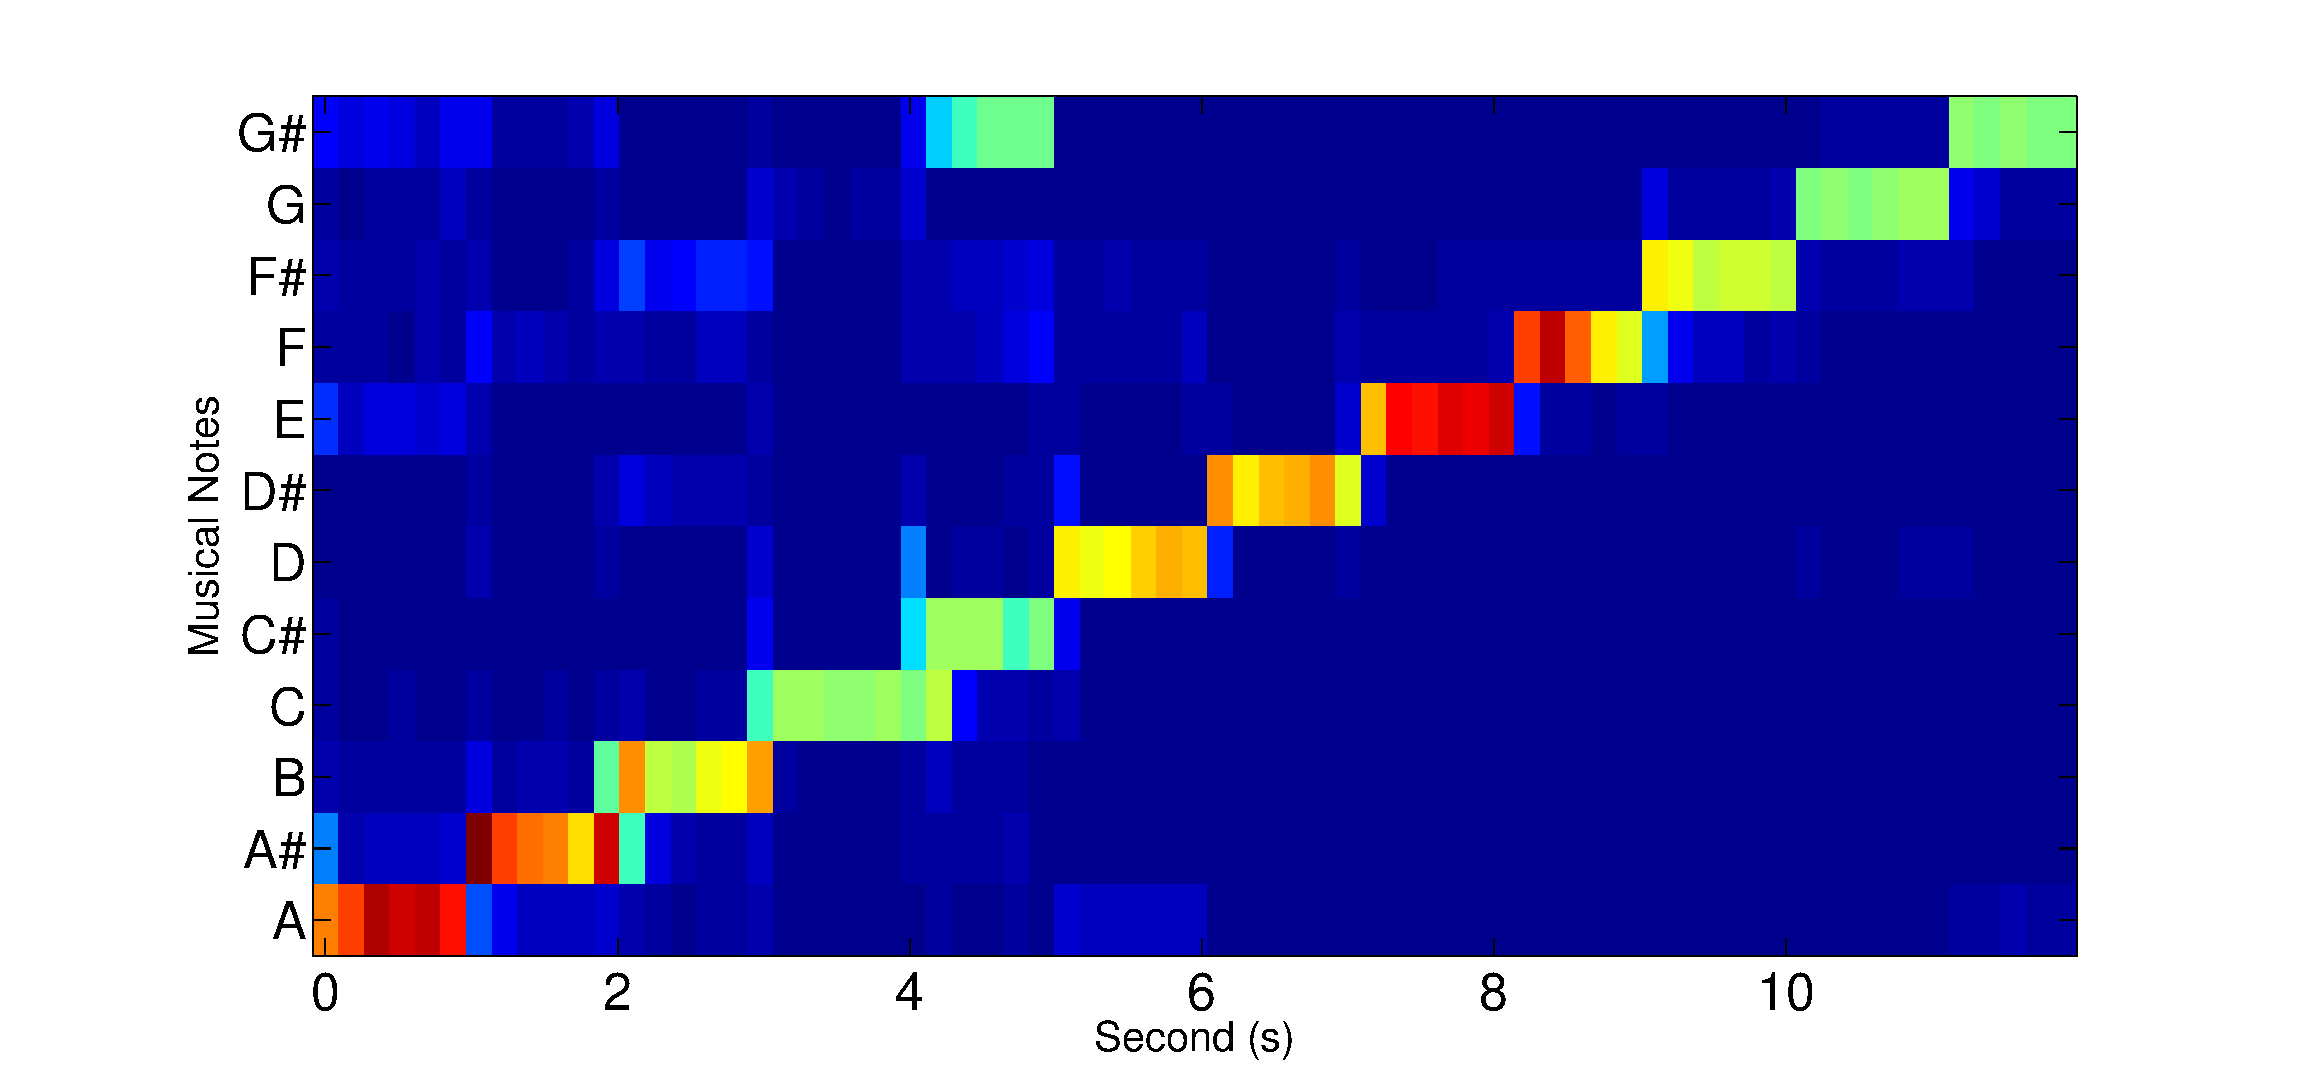
\includegraphics[width=\columnwidth, height=6cm]{figs/1-ccm.eps}}}
	 \caption{Obtained chroma feature by using the Chroma Convolution method.}
	 \label{fig:1-ccm}
	\end{figure}	



	

	\begin{table}[h!]
	 \begin{center}
	 \begin{tabular}{|l|l|}
	  \hline
	  Played Notes & Identified Notes \\
	  \hline
	  A  & A \\
	  A\#  & A\# \\
	  B  & B \\
	  C  & C \\
	  C\#  & C\# \\
	  C\#  & G\# \\
	  C\#  & C\# \\
	  D  & D \\
	  D\#  & D\# \\
	  E  & E \\
	  F  & F \\
	  F\#  & F\# \\
	  G  & G \\
	  G\#  & G\# \\
	  \hline
	 \end{tabular}
	\end{center}
	 \caption{Comparison between played and identified notes by the Chroma Convolution Method.}
	 \label{tab:table-1-ccm}
	\end{table}


	\subsection{Experiment 2: Identification of Musical Notes of Different Instruments}

	The second experiment is about the identification of tones of different instruments. For this to happen, the following melodies of the piano and the acoustic guitar were played together, as represented on \figref{fig:2-melodias}.

	\begin{figure}[h!]
	 \centerline{\framebox{
	 \includegraphics[width=\columnwidth]{figs/1-notes.png}}}
	 \centerline{\framebox{
	 \includegraphics[width=\columnwidth]{figs/2-notes-violao.png}}}
	 \centerline{\framebox{
	 \includegraphics[width=\columnwidth]{figs/2-notes-violao-piano.png}}}
	 \caption{The first sheet music is only piano, the second sheet music is only acoustic guitar and the third sheet music is the both together.}
	 \label{fig:2-melodias}
	\end{figure}

In CCM results, convolution of 12 tones of the acoustic guitar and 12 tones of the piano of different frequencies was used, generating two chroma feature respectively, one for each instrument. Both proposal windows were set in the length of 0.120 seconds, and the samplings rate of the audio was of 44.1 kHz.

	\subsubsection{STFT Results}
	In the following chroma feature was found using the traditional method of STFT on \figref{fig:2-ssft}. It can be observed on this picture that the chromatic scale of the piano was partially identified. The acoustic guitar tones are practically unnoticeable. 
	
	
	\begin{figure}[h!]
	 \centerline{\framebox{
	 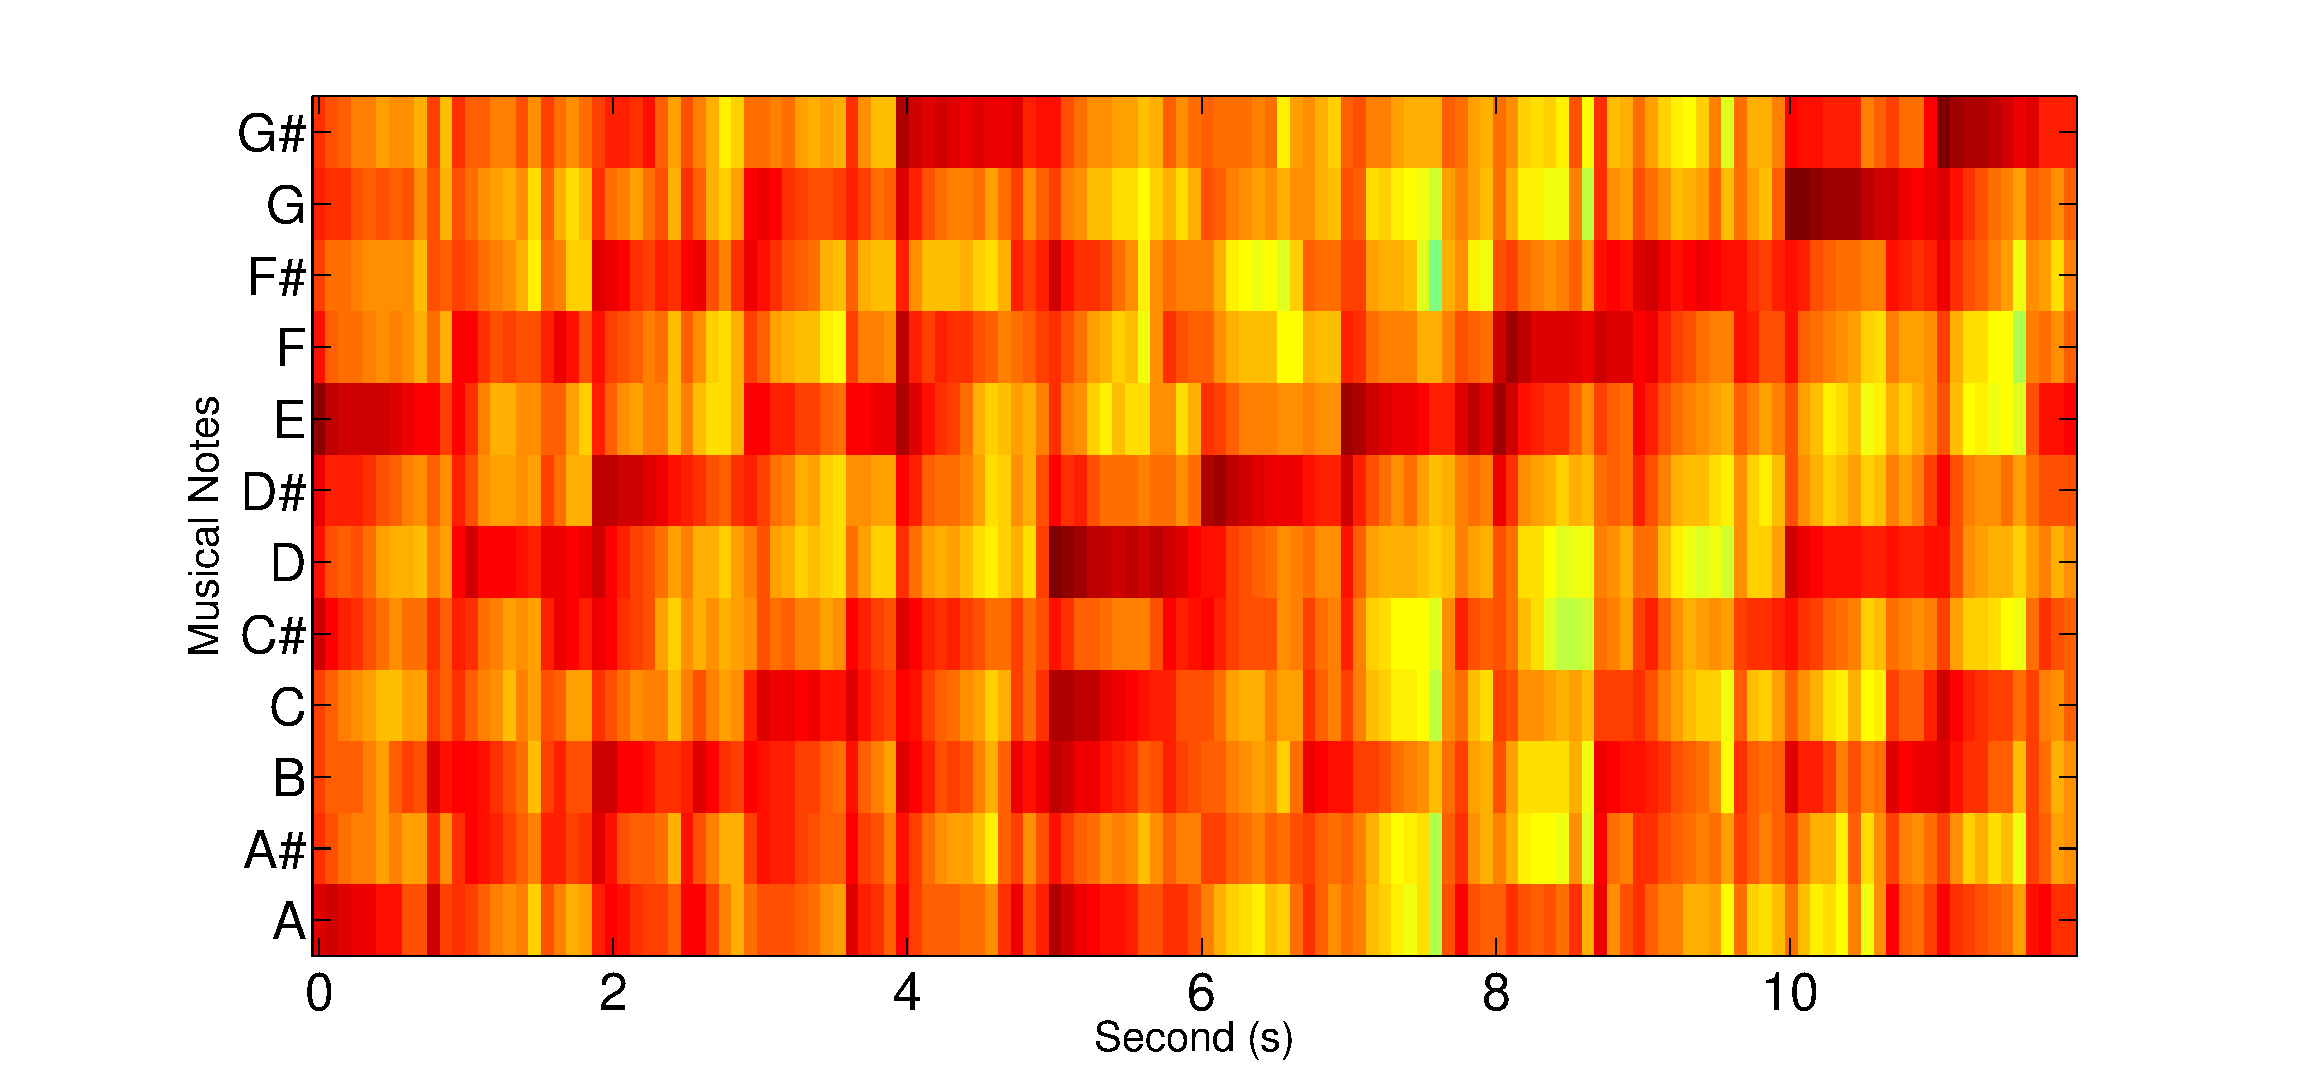
\includegraphics[width=\columnwidth, height=6cm]{figs/2-sfft.eps}}}
	 \caption{Chroma feature of audio using STFT.}
	 \label{fig:2-ssft}
	\end{figure}	

	It was also made an efficiency analysis on the recorded tones of the two instruments, with the sequence of identified tones in the chroma feature, using highest intensity in each minute-time. In the following the comparative table of \tabref{tab:table-2-sfft}.

	\begin{table}[h!]
	 \begin{center}
	 	\centerline{
	 \includegraphics[width=\columnwidth,height=9cm]{figs/tabela_2.png}}
	 \end{center}
	 \caption{Comparison between played notes of piano, acoustic guitar and identified by the STFT method.}
	 \label{tab:table-2-sfft}
	\end{table}


	First of all it is important to highlight that it is not possible to obtain a chroma feature for each instrument using the STFT method. This way, using an extraction of the tone of the chroma feature with more intensity in each minute-time, it was possible to obtain a value of the global efficiency, about 38.7\%, so, in each moment of time one of the two tones played by the instruments, piano and acoustic guitar, should be identified. The results of this analysis are on \tabref{tab:table-2-sfft}.

%-------------------------------------------------------------------
	\subsubsection{CCM Results}
	In the following chroma feature found using the traditional method using CCM of piano tones on \figref{fig:2-ccm-piano}.
	
	\begin{figure}[h!]
	 \centerline{\framebox{
	 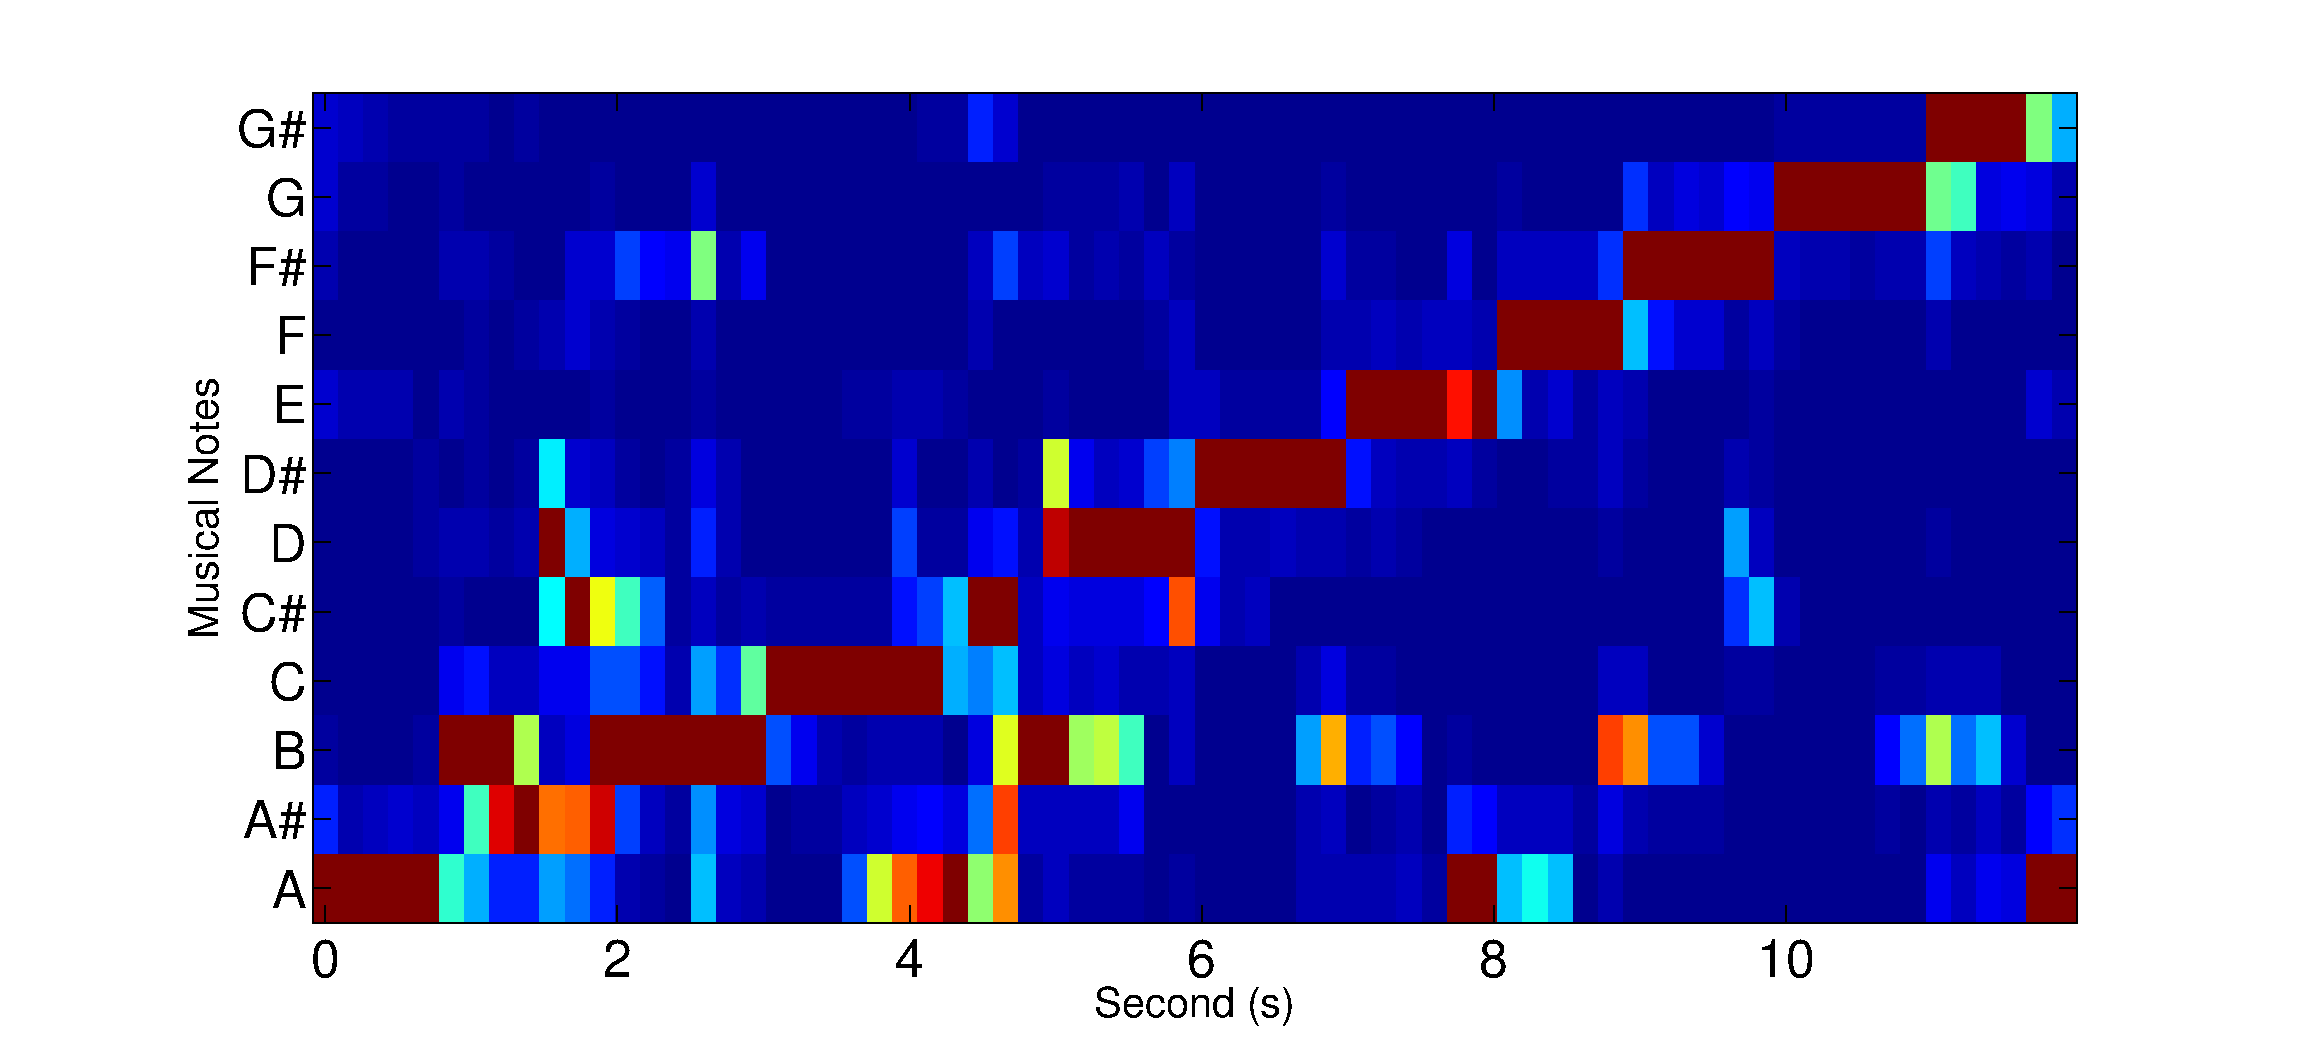
\includegraphics[width=\columnwidth, height=6cm]{figs/2-ccm-piano.eps}}}
	 \caption{Chroma feature of audio using CCM of piano tones.}
	 \label{fig:2-ccm-piano}
	\end{figure}	

	It can be observed that on \figref{fig:2-ccm-piano} the played melody of the piano was identified more clearly. It is also visible that some tones were executed by the acoustic guitar. A comparative table of the tones played and identified was made, also through the extraction of the tone of the chroma feature with more intensity in each minute-time. According to the results of \tabref{tab:table-2-ccm-piano}, there were 13 out of 18 tones of the piano in correct minute-time, representing 72.2\% fidelity to the original melody. The guitar, on the other hand, resulted in 5 out of 18 tones in correct minute-time, so, 27.7\%. This result shows that in this experiment the CCM amplified the executed tones, in the case of the piano, and suppressed the tones played by the acoustic guitar. 

	\begin{table}[h!]
	 \begin{center}
	 \begin{tabular}{|l|l|l|}
	  \hline
	  Piano & Acoustic Guitar & Identified Notes \\
	  \hline
		A	& A	& A \\
		A	&    B	&    B \\
		A\#	&    B	&    A\# \\
		A\#	&    B	&    C\# \\
		A\#	&    C\#	&    A\# \\
		B	&    B	&    B \\
		C	&    A	&    C \\
		C\#	&    A	&    A \\
		C\#	&    B	&    C\# \\
		D	&    B	&    B \\
		D	&    C\#	&    D \\
		D\#	&    B	&    D\# \\
		E	&    A	&    E \\
		F	&    B	&    F \\
		F\#	&    C\#	&    F\# \\
		G	&    B	&    G \\
		G\#	&    B	&    G\# \\
		G\#	&    B	&    A \\
	  \hline
	 \end{tabular}
	\end{center}
	 \caption{Comparison between played notes of piano, acoustic guitar and identified notes by the CCM with piano tones.}
	 \label{tab:table-2-ccm-piano}
	\end{table}


In the following chroma feature found using the CCM of tones of the acoustic guitar on \figref{fig:2-ccm-violao}. It can be observed on the picture that the melody executed by the acoustic guitar was also identified more clearly. Some tones of the chromatic scale executed by the piano are visible as well, although suppressed if in contrast with the result presented on \figref{fig:2-ccm-piano}. A comparative table of the tones which were played and identified was also made through the extraction of the tone of the chroma feature with more intensity in each minute-time. As it is seen on \tabref{tab:table-2-ccm-violao}, 9 out of the 19 tones executed by the acoustic guitar were identified correctly, so, 47.4\% fidelity to the original melody. Talking about the piano, 2 out of 19 tones were identified correctly, representing 10.5\%. 
	
	\begin{figure}[h!]
	 \centerline{\framebox{
	 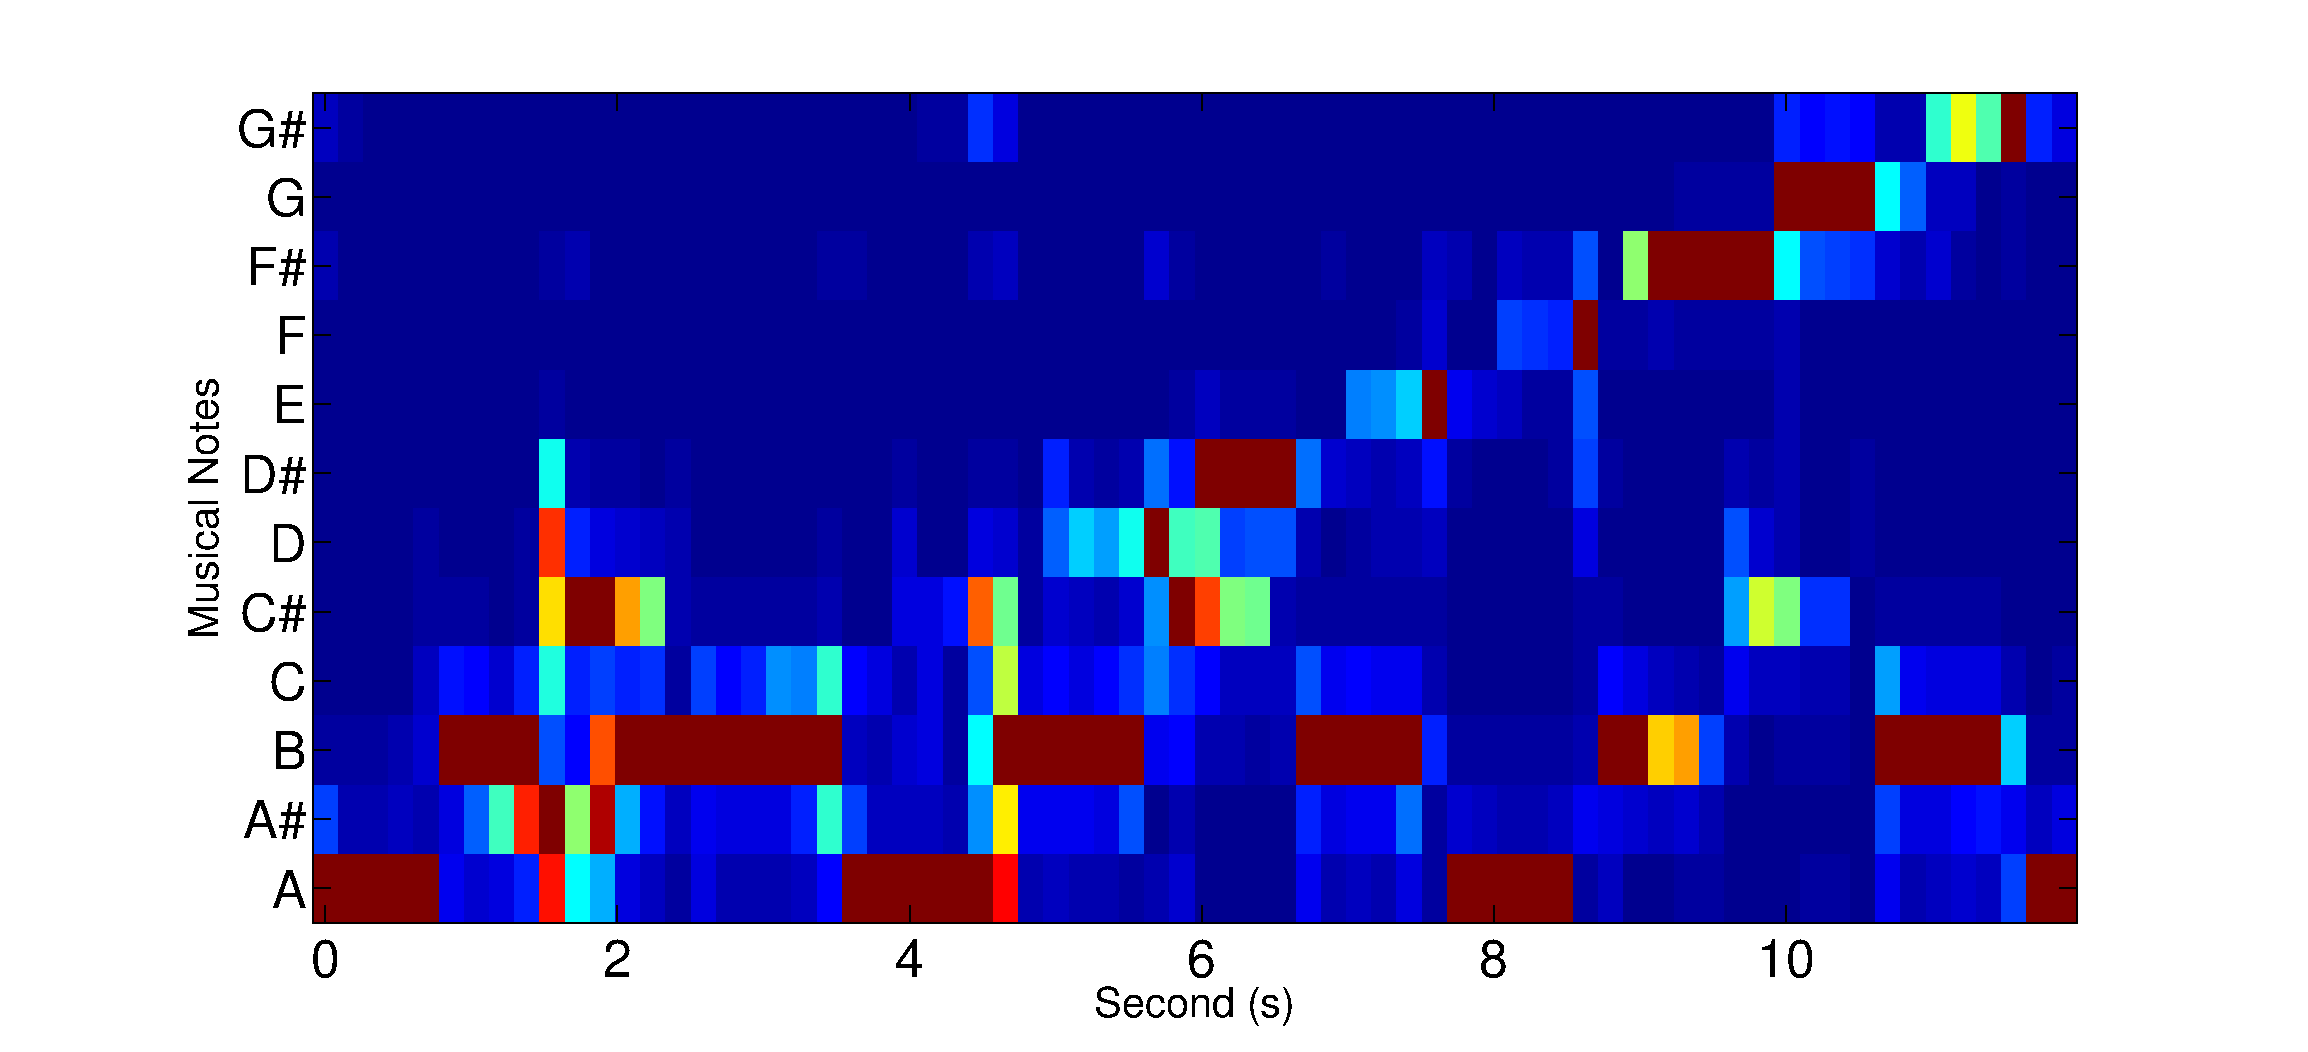
\includegraphics[width=\columnwidth, height=6cm]{figs/2-ccm-violao.eps}}}
	 \caption{Chroma feature of audio using CCM of acoustic guitar tones.}
	 \label{fig:2-ccm-violao}
	\end{figure}	


	\begin{table}[h!]
	 \begin{center}
	 \begin{tabular}{|l|l|l|}
	  \hline
	  Piano & Acoustic Guitar & Identified Notes \\
	  \hline
			  A & A &  A \\
		A\# &  B &  B \\
		    A\# &  B &    A\# \\
		    B  &   C\# &  C\# \\
		    C   &  B  &   B \\
		    C\# &  A   &  A \\
		    D   &  B   &  C\# \\
		    D\# &  C\# &  B \\
		    D\# &  C\# &  D \\
		    D\# &  C\# &  C\# \\
		    E   &  B  &   D\# \\
		    F   &  A   &  B \\
		    F   &  A  &   E \\
		    F\# &  B  &   A \\
		    F\# &  B   &  B \\
		    G   &  C\# &  F\# \\
		    G   &  C\# &  C\# \\
		    G\# &  B   &  G \\
		    G\# &  B  &   B \\
	  \hline
	 \end{tabular}
	\end{center}
	 \caption{Comparison between played notes of piano, acoustic guitar and identified notes by the CCM with acoustic guitar tones.}
	 \label{tab:table-2-ccm-violao}
	\end{table}


\section{Discussion}\label{sec:discussion}

	The results reached by CCM are more satisfactory than the traditional method STFT, although a largest computational cost is attained to CCM calculations. The time of processing of the STFT method was approximately 0.1 seconds against 13.2 seconds of CCM in the first experiment. It has to be highlighted that the high computational cost of CCM does not represent a limitation in practical terms, as the method can be executed, without great problems, by a personal computer.

	In the first experiment, the CCM presented an improvement in its efficiency of about 28.6\% in relation to the traditional method. In a way, the CCM values the energy of the tones that have some correlation to the reference signal, what favor identification. Another important point is the fact that the CCM suppresses the signal information which is not correlated to the reference signals used in the convolution.

	Moreover, there is the possibility, offered by the CCM, of focusing the attention on an specific instrument, through the use of its timber, without any additional costs to the algorithm. Reference tones recorded by the piano were better identified in the second experiment, as the acoustic guitar tones were suppressed. The inverted result was observed when the same audio signal was submitted to the reference signals produced by the acoustic guitar. The order of magnitude found to the identification of the privileged tones for the reference signals in relation to the suppressed tones was about 40.7\%. The traditional method STFT does not offer the possibility, unless the optimizations start being practiced in order to consider the timber of the instruments in a similar way.


	\section{Conclusions and Future Works}\label{sec:conclusions}

	This paper presented a new way of constructing the chroma feature or PCP, from the use of a new method, here denominated chroma convolution method (CCM). The obtained results were confronted with the traditional algorithm STFT, showing more efficiency to the CCM when identifying musical tones.

	Another advantaged found to the CCM in relation to the traditional method STFT is about the detection of polyphonic melodies, produced by more than one instrument. The CCM operates with reference signals for the tones to be identified, what can be obtained from actual instruments, which naturally leads to the inclusion of information of timber of identification. 

	This paper presented a standard and basic way of CCM use, without any procedure for noise reduction or any improvement over the tone identification. In the same way that the traditional method STFT has been developed for more sophisticated applications, like the NNLS \cite{mauch2010approximate} and the particle filters \cite{jo2010melody}, the CCM method can be improved, aiming better results.
	
	It is worth mentioning that the CCM and the STFT methods were compared in their basic applications, so, there is a lot to be done, e.g. the submission and validation on MIREX, in the CCM strategy in what concerns the identification of tones and polyphonic melodies, considering the great amount of papers already produced by the traditional solutions in the frequency domain.


% For bibtex users:
\bibliography{ISMIR2015template}

% For non bibtex users:
%\begin{thebibliography}{citations}
%
%\bibitem {Author:00}
%E. Author.
%``The Title of the Conference Paper,''
%{\it Proceedings of the International Symposium
%on Music Information Retrieval}, pp.~000--111, 2000.
%
%\bibitem{Someone:10}
%A. Someone, B. Someone, and C. Someone.
%``The Title of the Journal Paper,''
%{\it Journal of New Music Research},
%Vol.~A, No.~B, pp.~111--222, 2010.
%
%\bibitem{Someone:04} X. Someone and Y. Someone. {\it Title of the Book},
%    Editorial Acme, Porto, 2012.
%
%\end{thebibliography}

\end{document}
